\chapter[Paper: LSTM Network Behaviour for IMU Based Locomotion Mode Recognition Systems]{Understanding LSTM Network Behaviour of IMU-Based Locomotion Mode Recognition for Applications in Prostheses and Wearables}
\label{chp:lstm-general}

\section{Introduction and commentary}
% Where possible please ensure that the page numbers tie in with the rest of the thesis document, 
% where this is not possible, you should insert an extra page before the academic paper which shows 
% the citation details and gives the page numbers of the thesis that the academic paper covers.
% \usepackage{graphicx}
% \usepackage{colortbl}
\newcommand\x{\value{page}}
Pleas note: This paper contains duplication of material presented is Chapters \ref{chp:background} and \ref{chp:methods}. The paper contains both the page numbers as originally published and thesis page numbering. The paper covers thesis pages \the\numexpr\x+2\relax \ to \the\numexpr\x+24\relax

\clearpage
\section{Authorship and permissions}
% \newcommand{\backgoundColor}{0.871,0.918,0.965}
\newcommand{\backgoundColor}{1,1,1}
\newcommand{\boxColor}{0.95,0.95,0.95}

{\begin{table}[!hbt]
\caption{Statement of Authorship}
\ 

\hyphenpenalty=10000
\begin{tabularx}{\textwidth}{>{\raggedright}p{1.5in}X}
\hline
\rowcolor[rgb]{\backgoundColor}
\multicolumn{2}{l}{\textbf{This declaration concerns the article entitled:}}\\
\hline
\multicolumn{2}{p{0.9\textwidth}}{Understanding LSTM Network Behaviour of IMU-Based Locomotion Mode Recognition for Applications in Prostheses and Wearables} \\

\hline
\rowcolor[rgb]{\backgoundColor}
\multicolumn{2}{l}{\textbf{Publication status (tick one)}}  \\
\rowcolor[rgb]{\backgoundColor}
\multicolumn{2}{l}{\begin{tabular}{rcrcrcrcrc}
    \textbf\ {Draft} &{\cellcolor[rgb]{\boxColor}} \ &
    \textbf{\ Submitted} &{\cellcolor[rgb]{\boxColor}} \ &
    \textbf{\ In review} &{\cellcolor[rgb]{\boxColor}} \ &
    \textbf{\ Accepted} &{\cellcolor[rgb]{\boxColor}} \ &
    \textbf{\ Published} &{\cellcolor[rgb]{\boxColor}}X 
\end{tabular}}  \\
\rowcolor[rgb]{\backgoundColor}\multicolumn{2}{l}{} \\

% Publication details
\hline
{\cellcolor[rgb]{\backgoundColor}}\textbf{Publication details (reference)} & Sensors 2021, 21, 1264.

\ 

DOI: \href{https://doi.org/10.3390/s21041264}{10.3390/s21041264} 

\ 

Received: 23 December 2020, Accepted: 6 February 2021, Published: 10 February 2021\\


\hline
\rowcolor[rgb]{\backgoundColor}
\multicolumn{2}{l}{\textbf{Publication status (tick one)}} 

\\
\rowcolor[rgb]{\backgoundColor}
\multicolumn{2}{l}{\begin{tabular}{rcrc}
    \textbf{I hold the copyright} &{\cellcolor[rgb]{\boxColor}} \ &
    \textbf{\ Copyright is retained by the publisher, but} &{\cellcolor[rgb]{\boxColor}}X \\
    \textbf{for this material}& & \textbf{I have been given permission to replicate} & \\
    & & \textbf{ the material here} & \\
\end{tabular}}  \\
\rowcolor[rgb]{\backgoundColor}\multicolumn{2}{l}{} \\

\hline
{\cellcolor[rgb]{\backgoundColor}}\textbf{Candidate’s contribution to the paper (provide details, and also indicate as a percentage)} & The candidate contributed to / considerably contributed to / predominantly executed the…

\ 

\textbf{Formulation of ideas: (95\%)}

The experiment and analysis methodology was conceived by Freddie Sherratt with supervision from Pejman Iravani

\ 


\textbf{Design of methodology: (95\%)}

The experiment and analysis methodology was conceived by Freddie Sherratt with supervision from Pejman Iravani

\ 


\textbf{Experimental work: (95\%)}

The experimental work was carried out entirely by Freddie Sherratt with supervision from Pejman Iravani

\ 


\textbf{Presentation of data in journal format: (95\%)}

The data presentation was carried out entirely by Freddie Sherratt with supervision from Pejman Iravani and Andrew Plummer

\\

\hline
{\cellcolor[rgb]{\backgoundColor}}\textbf{Statement from Candidate} &
This paper reports on original research I conducted during the period of my Higher Degree by Research candidature.\\

\hline
{\cellcolor[rgb]{\backgoundColor}}\textbf{Signed} & Freddie Sherratt 
{\begin{tabular}{p{0.6in}ll}
     \ & {\cellcolor[rgb]{\backgoundColor}}\textbf{\ \ Date } & 4th March 2021 
\end{tabular}}\\
\hline
\end{tabularx}
\end{table}}

\clearpage

% Paper
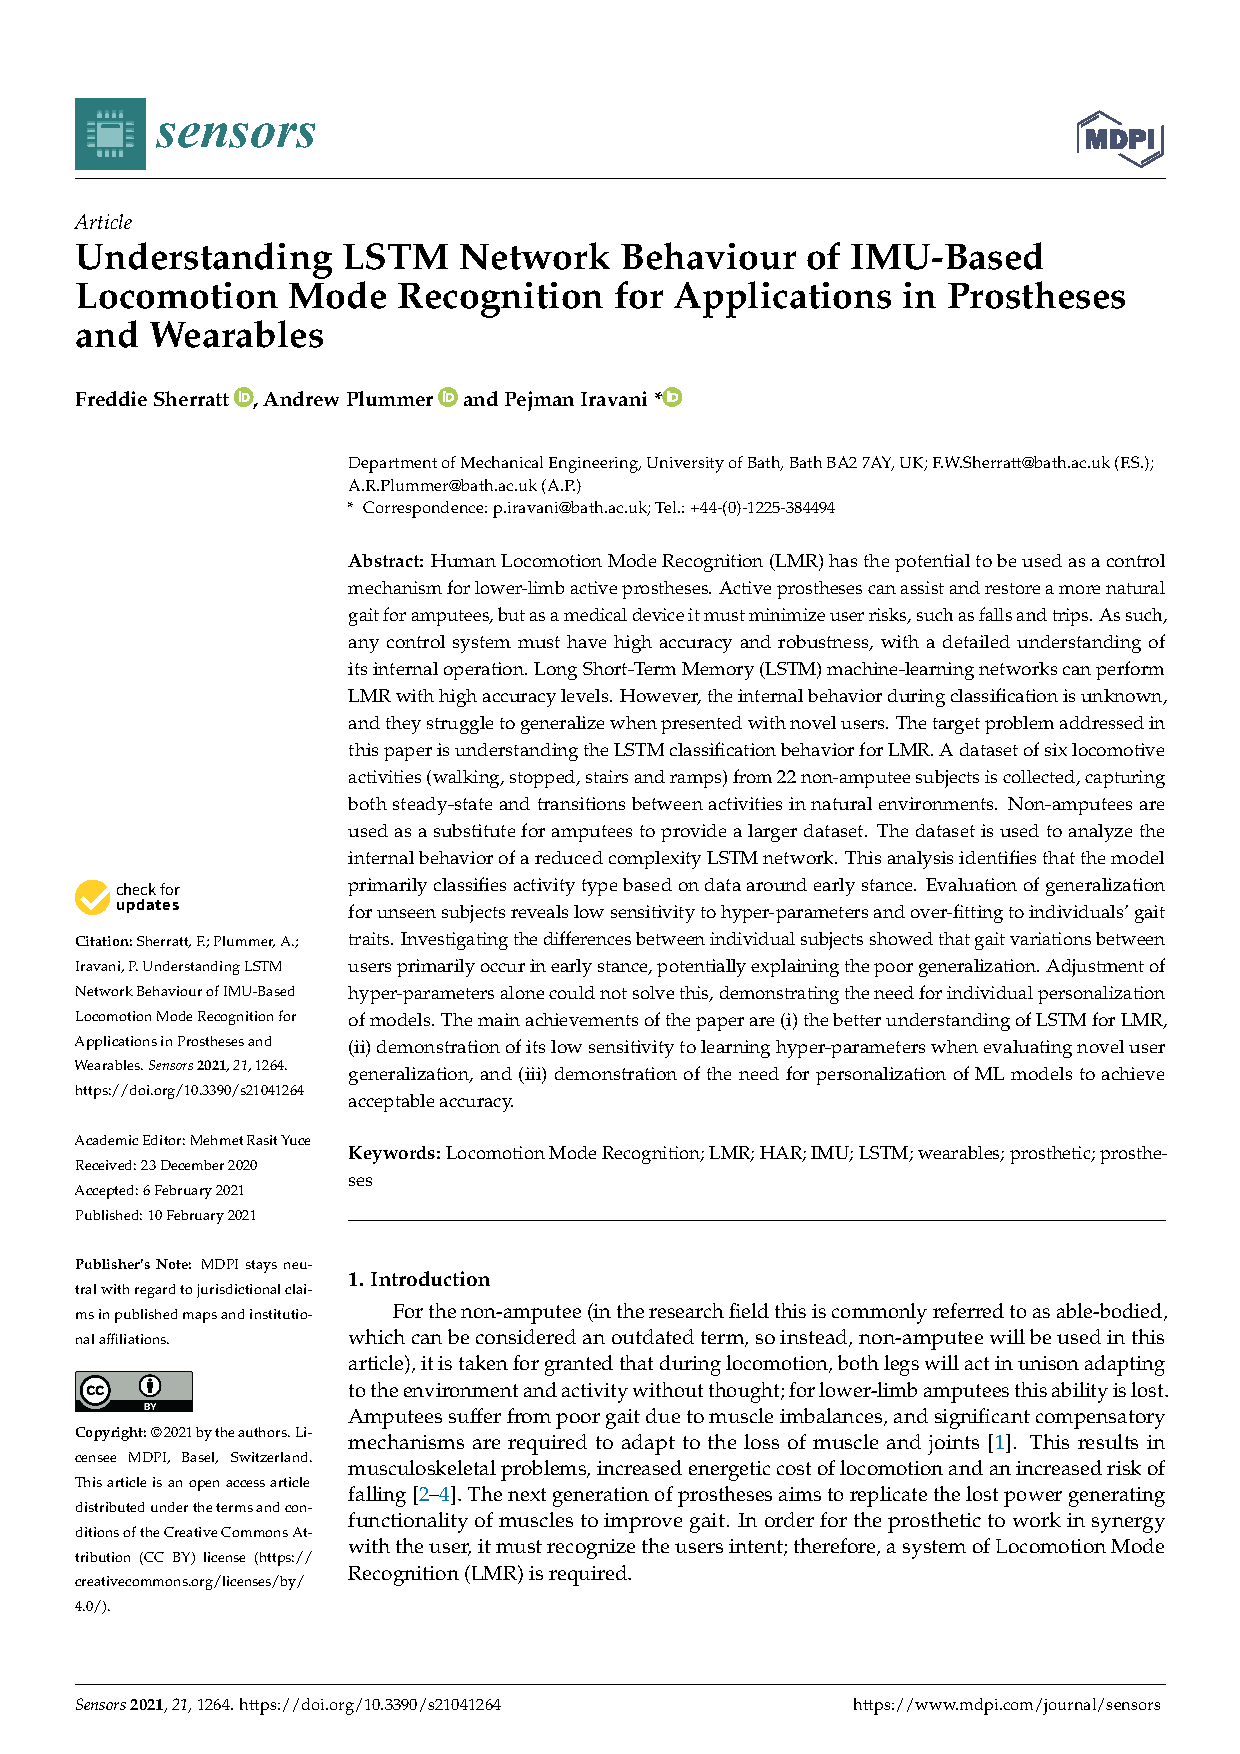
\includepdf[pages=-,scale=.83,offset=11mm 8mm,pagecommand={\thispagestyle{fancy}}, frame=false]{content/4-LSTM_Behaviour/sensors-21-01264-v2.pdf}

\clearpage


% \setcounter{page}{\numexpr\x + 23\relax}

\section{Post-commentary}
Since being published, this paper has received a number of citations

What was the big takeaway from this paper - demonstrates the need for personalisation
